%!TEX root = ../thesis.tex
%*******************************************************************************
%****************************** Second Chapter *********************************
%*******************************************************************************

\chapter{Preliminaries and state of the art}

\ifpdf
    \graphicspath{{Chapter2/Figs/Raster/}{Chapter2/Figs/PDF/}{Chapter2/Figs/}}
\else
    \graphicspath{{Chapter2/Figs/Vector/}{Chapter2/Figs/}}
\fi

In this chapter, some mathematical preliminaries that will be used throughout the document are presented. The first part is focused on the image processing. After it is explained the basic concepts of projective geometry, and it is made an analysis of the model geometry. Although this work considers that the intrinsic and extrinsic parameters are known, an introduction of the techniques of calibration of the camera is written in this part. In the second section of the chapter there is an overview of the mini-helicopter four-rotor UAVs, and in the same way the dynamic model is detailed.

 \section{Computer Vision}
 \subsection{Projective geometry}
 \subsection{Model geometry}
 \subsection{Camera calibration}
 \subsection{Formation of the image in projective geometry}



 \section{UAVs: Mini-helicopter of four rotors}

 An Unmanned Aerial Vehicle (UAV) is an autonomous flying machine, this means that the vehicle can perform flights without a human pilot by the usage of an autonomous pilot algorithm. While the concept of UAV seems a novelty, its usage is not. In fact, the interest in the study of these type of vehicles has increased, and there are many works published especially related to control laws applied on the topic. The research on this subject is also possible due to the evolution of information and communication technologies and the power computation of the different devices.

It should be noted that the ballistic or semi-ballistic missiles, the cruise missiles and the artillery projectiles are not considered UAV systems.

An UAV system is composed mainly by two elements:
\begin{itemize}
  \item Flight component: formed by the aerial vehicle.
  \item Ground component: formed by the ground station, which allows the communication between this and the aerial system, data processing, monitoring, control, etc.
\end{itemize}

In general the drones can be classified according with the size, the application or a combination of both, however, the size is the most used criterion to make the classification. The classification, depicted in \fig{fig:categories} is resumed in the next items, \cite{phdguerrero:2008}:
\begin{itemize}
  \item Micro-UAV: This kind of vehicles can be operated by just one person. The propulsion is electrically made and due to the low cost of the materials, the vehicles are primarily used for civilian applications. The average autonomy is about 30 minutes.
  \item Mini-UAV: The equipment necessary for these vehicles is more specialized. In general, these drones fly at speeds of $70km/h$ and medium altitudes of $3,5km$. Their size allows them to fly around 4 hours.
  \item MALE/HALE: The Medium Altitude High Endurance (MALE) drones are used to perform higher endurance flights and also at higher altitudes ($10-15km$). The High Altitude High Endurance (HALE) drones can fly at about $20km$ of altitude. These drones are able to perform missions with medium endurance of two days. The Predator (MALE) and the Global Hawk (HALE) are the most popular drones of this category and are mainly applied for military missions.
  \item UCAV: The Unmanned Combat Air Vehicle is mainly used for offensive missions. They are under research and only some prototypes are available, like the RQ-170 Centinel.
\end{itemize}


\begin{figure}[H]
    \centering
    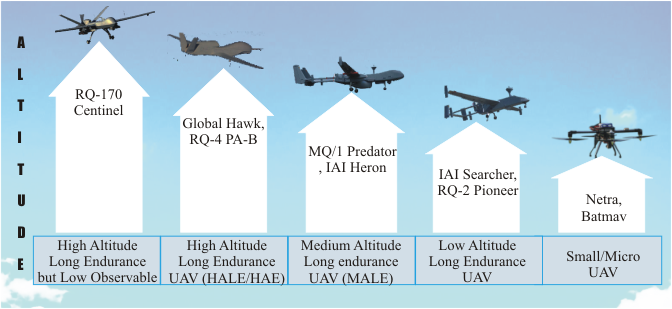
\includegraphics[width =\textwidth]{figures/categories.png}
    \caption{The different categories of drones.}
    \label{fig:categories}
  \end{figure}

Due to their aerodynamical function, there is an alternative classification, where it is possible to find three families: fixed wings aircrafts, rotating wings aircrafts and the swing-wing aircrafts. A study shows that the research has mainly focused on the rotating wings aircrafts with VTOL (Vertical Take Off and Landing) configuration. These vehicles are capable of take off and land in a vertical way and due to this advantage, the range of applications is very extensive, being used on military and civilian applications, like surveillance, rescue, aerial mapping, etc.

 \subsection{Vertical Take Off and Landing (VTOL) vehicles}
 \subsection{Rotorcraft}
\begin{itemize}
  \item Helicopter: is a type of rotorcraft in which lift and thrust are supplied by rotors. This allows the helicopter to take off and land vertically, to hover, and to fly forward and laterally. These attributes allow helicopters to be used in congested or isolated areas where fixed-wing aircrafts would usually not be able to take off or land.\fig{apache} shows an example of a helicopter.

      \begin{figure}[h!]
        \centering
        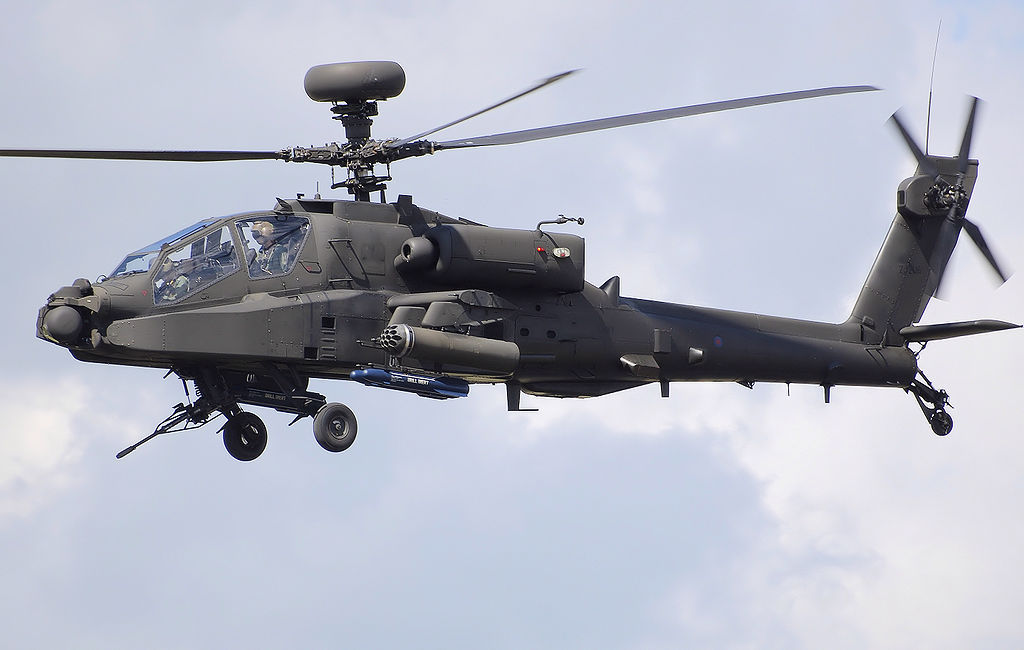
\includegraphics[width=0.4\textwidth]{figures/apache.jpg}
        \caption{An Apache attack helicopter}\label{apache}
      \end{figure}

  \item Multirotor: also called multicopter, is a rotorcraft with more than two rotors. An advantage of multirotor aircraft  is the simpler rotor mechanics required for flight control. Unlike single and double-rotor helicopters, multirotors often use fixed-pitch and yaw blades; control of vehicle motion is achieved by varying the relative speed of each rotor to change the thrust and torque produced by each one. Due to their ease of both construction and control, multirotor aircraft are frequently used in radio control aircraft and UAV projects, in which the names \textbf{tricopter}, \textbf{quadcopter} see \fig{fig:quaddji}, \textbf{hexacopter} and \textbf{octocopter} see \fig{fig:octodji}, are frequently used to refer to 3, 4, 6 and 8-rotor helicopters, respectively.
%
  \begin{figure} [h!]
\centering
% \begin{multicols}{2}
\begin{subfigure}[t]{0.45\textwidth}
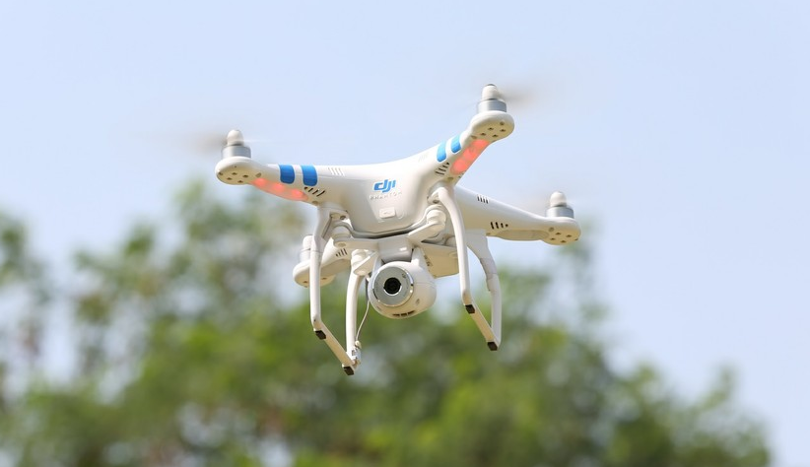
\includegraphics[width = \textwidth]{figures/quaddji.png}
\caption{}
\label{fig:quaddji}
\end{subfigure}
%$\qquad$
%\hfill
\begin{subfigure}[t]{0.45\textwidth}
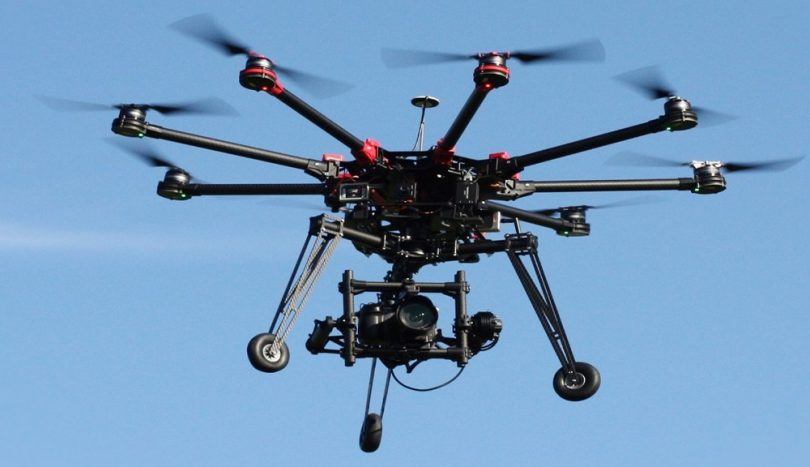
\includegraphics[width = \textwidth]{figures/octodji.jpg}
\caption{}
\label{fig:octodji}
\end{subfigure}
\caption{(a)Quadcopter and (b)octocopter configurations, courtesy of (\cite{website:dji})}
  \label{fig:multirotor}
\end{figure}

%
\item Autogyro: is also known as gyroplane, gyrocopter or rotaplane. Is a type of rotorcraft that uses an unpowered rotor in autorotation to develop lift, and an engine-powered propeller, similar to that of a fixed-wing aircraft, to provide thrust. While similar to a helicopter rotor in appearance, the autogyro's rotor must have air flowing through the rotor disc to generate rotation. \fig{auto} shows an example of an autogyro.

      \begin{figure}[h!]
        \centering
        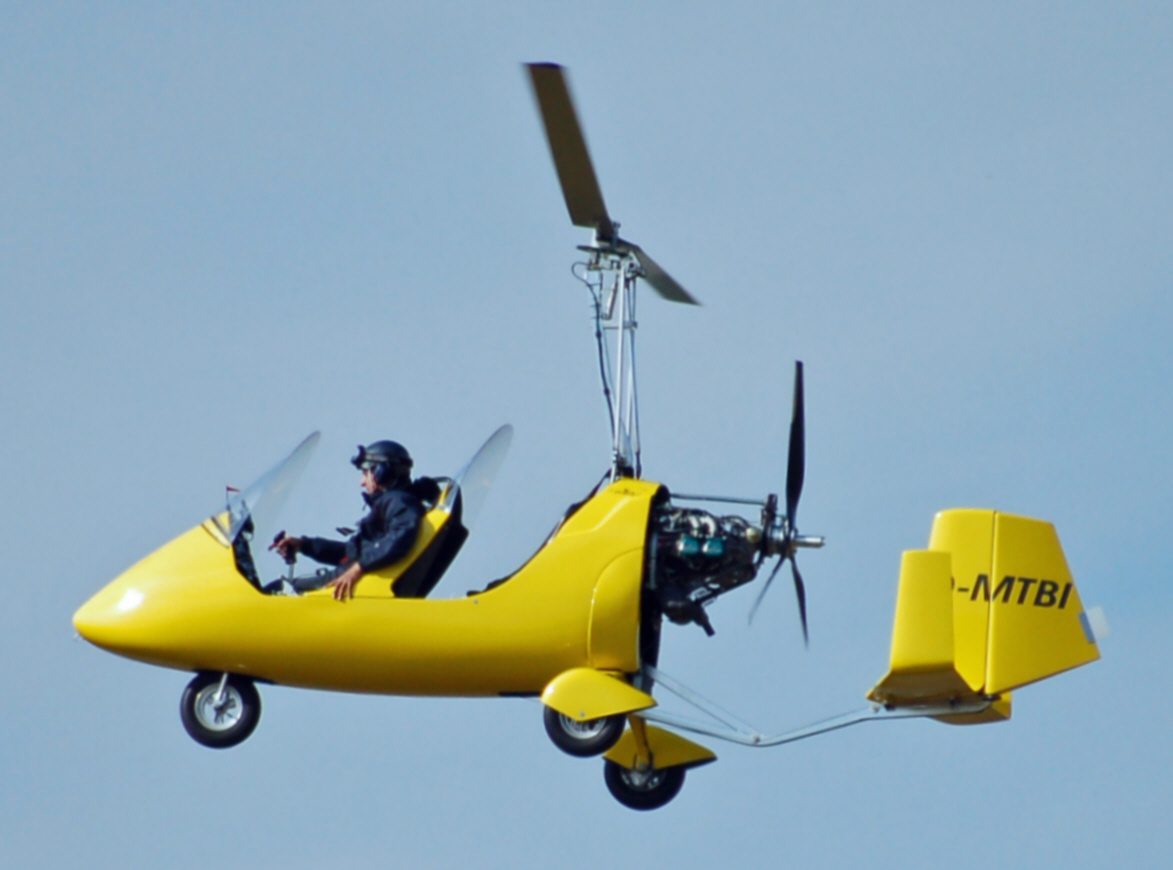
\includegraphics[width=0.4\textwidth]{figures/autogyro.jpg}
        \caption{Autogyro MT-03 in flight}\label{auto}
      \end{figure}

  \item Gyrodyne: is a type of VTOL aircraft with a helicopter rotor-like system that is driven by its engine for take off and landing and also includes one or more conventional propellers to provide forward thrust during cruising flight. Lift during forward flight is provided by a combination of the rotor, like the autogyro, as well as conventional wings.

   \fig{gyro} shows an example of gyrodyne.
      \begin{figure}[h!]
        \centering
        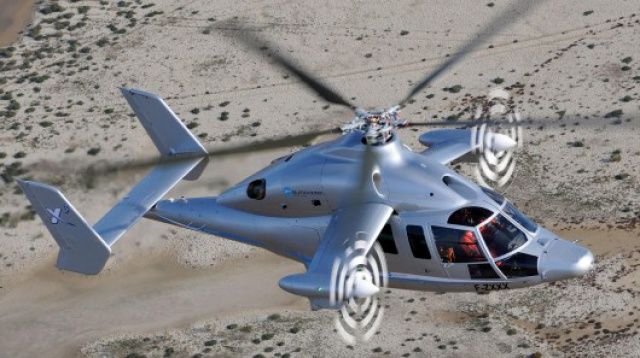
\includegraphics[width=0.45\textwidth]{figures/gyro.jpg}
        \caption{Gyrodyne AM-X3 in flight}\label{gyro}
      \end{figure}

\end{itemize}

\subsection{Powered lift}
\begin{itemize}
  \item Convertiplane: is an aircraft which uses rotor power for vertical take off and landing and converts to fixed-wing lift in normal flight. These vehicles may be divided into two broad classes, based on wether the rotor is fixed as in a helicopter or tilts to provide thrust in forward flight. \fig{convert} shows an example of a convertiplane.

      \begin{figure}[h!]
        \centering
        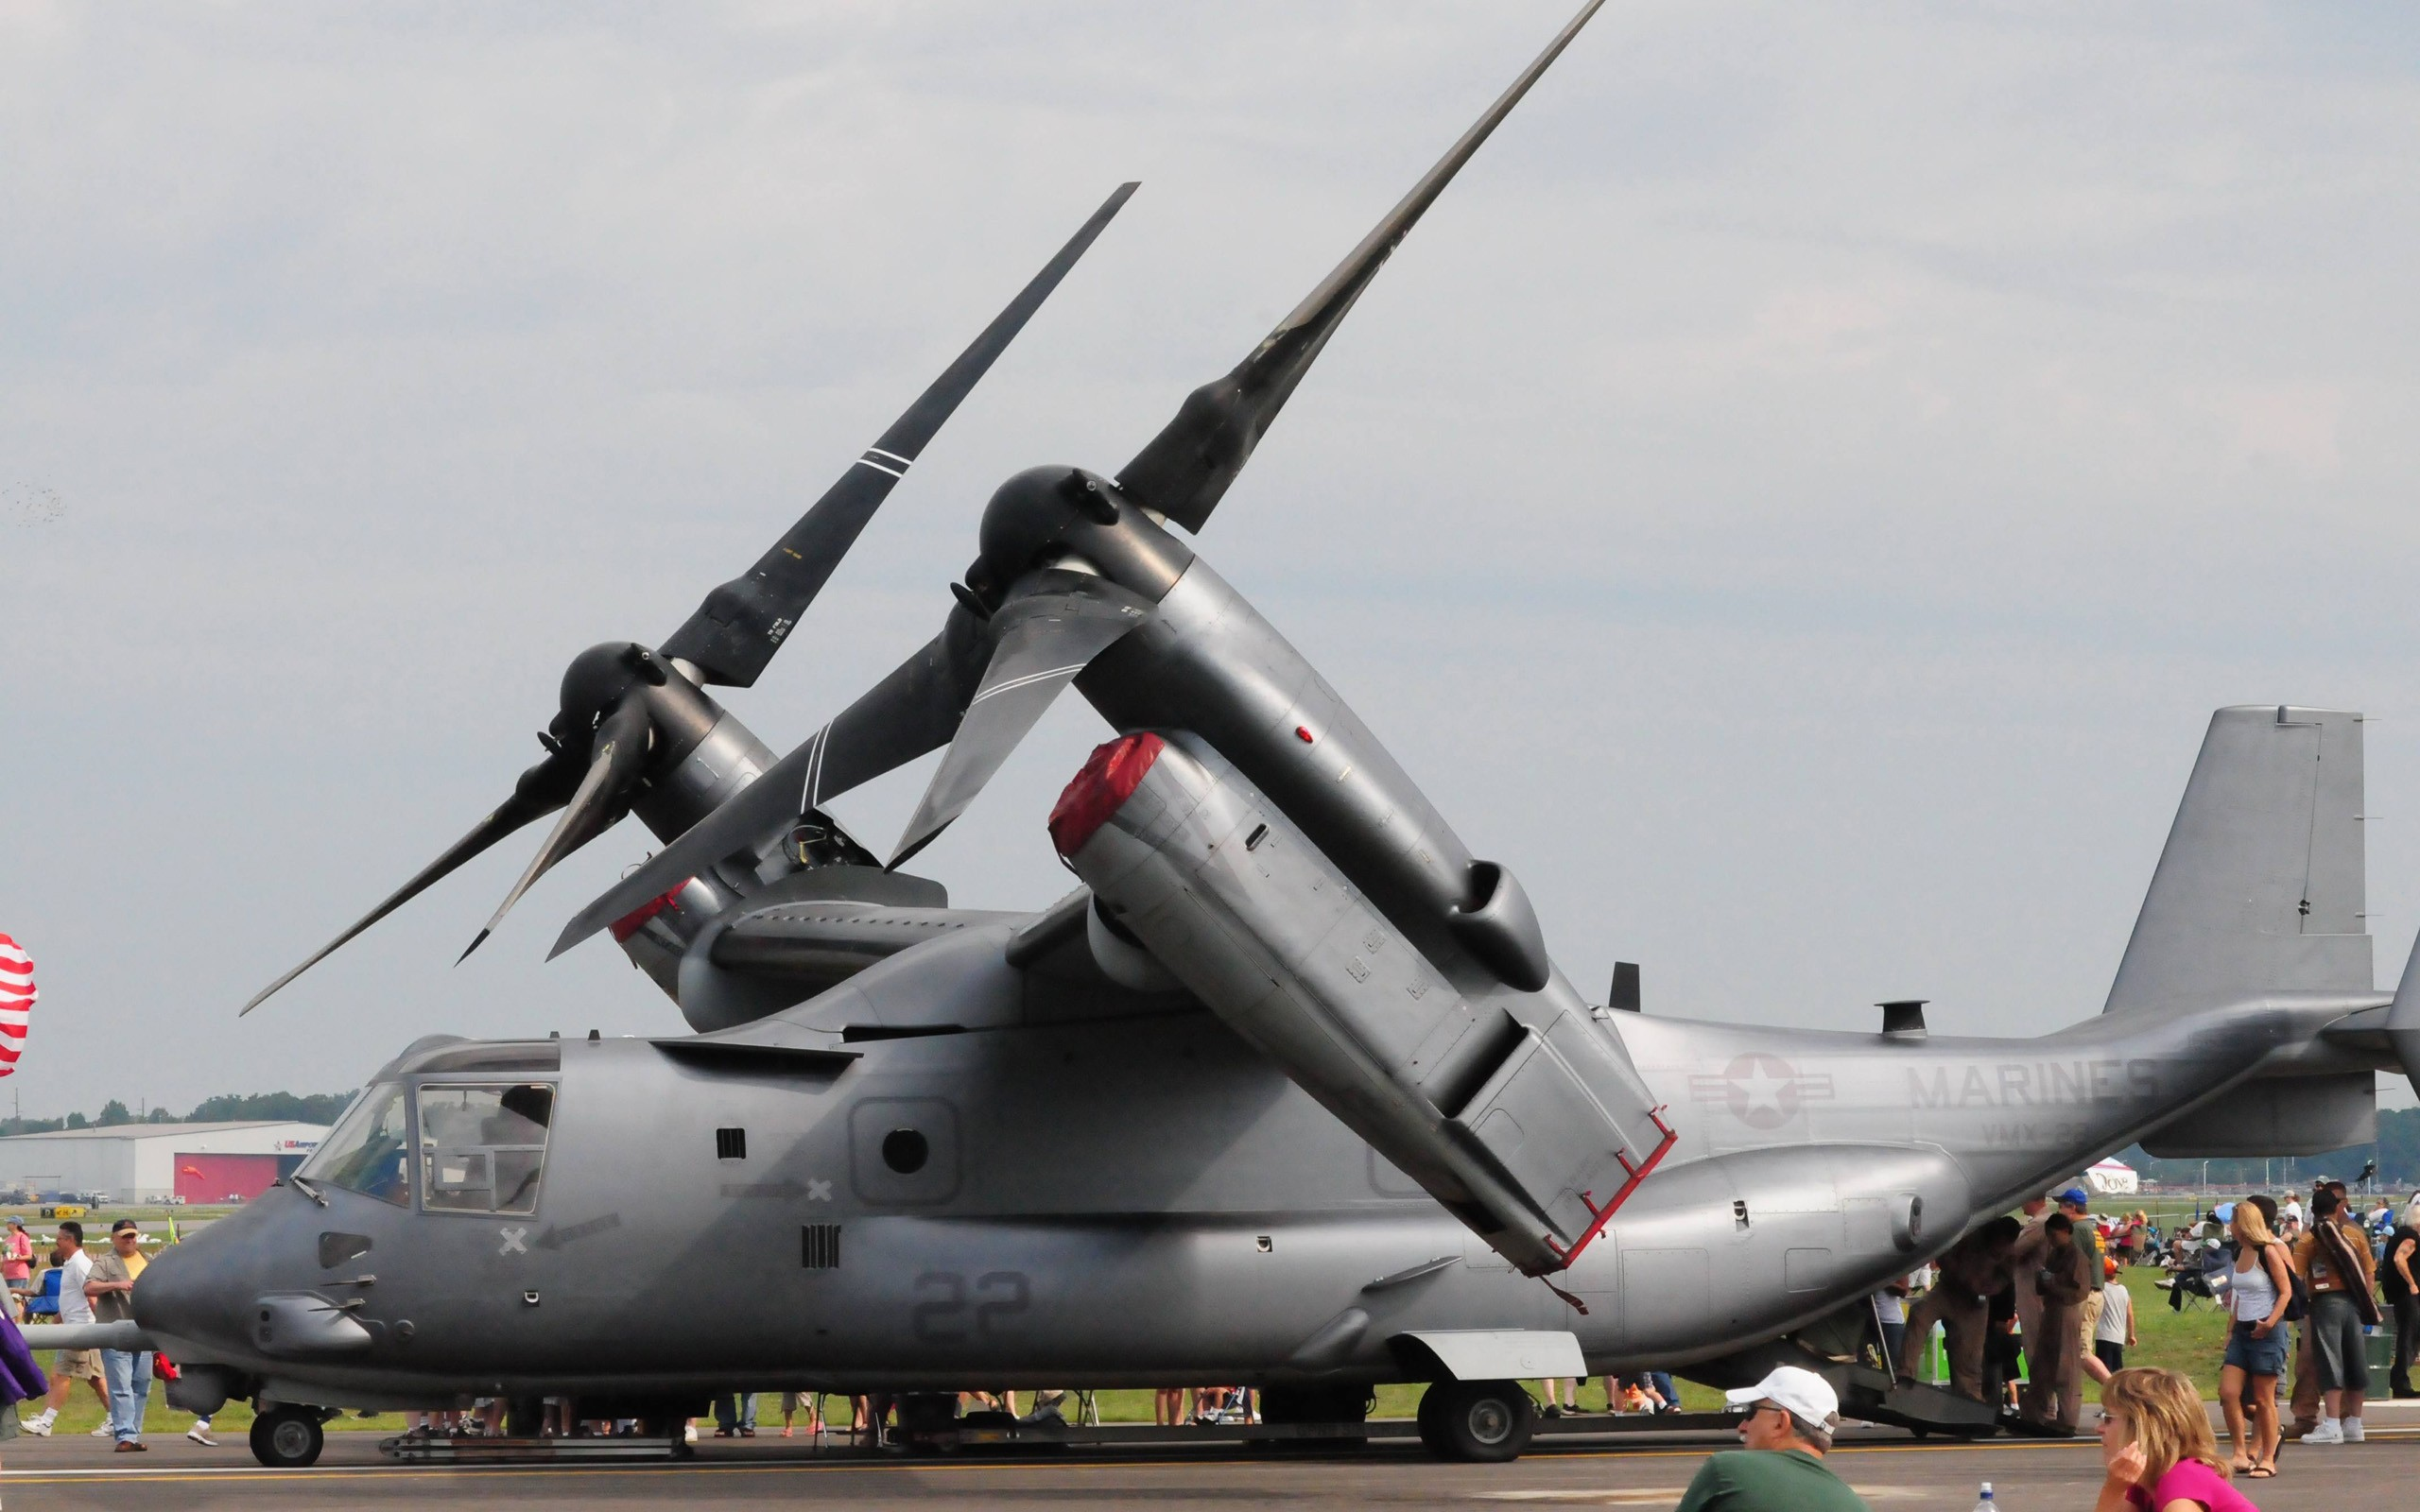
\includegraphics[width=0.4\textwidth]{figures/converti.jpg}
        \caption{Convertiplane}\label{convert}
      \end{figure}

  \item Tail-sitter: called also tailsitter, is a type of VTOL vehicle that takes off and lands on its tail, then tilts horizontally for forward flight. \fig{tail} shows an example of tail-sitter UAV's.

      \begin{figure}[h!]
        \centering
        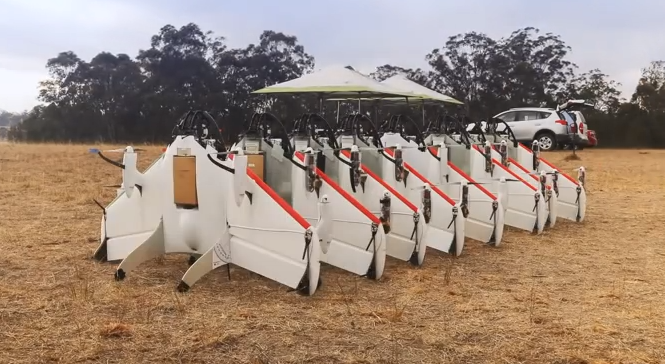
\includegraphics[width=0.45\textwidth]{figures/tail.png}
        \caption{Tail-sitter prototypes, as part of the Google’s project Wing for delivery}\label{tail}
      \end{figure}

  \item Lift jets: is an auxiliary jet engine used to provide lift for VTOL operation, but may be shut down for normal wing-borne flight.
  \item Lift fans: is an aircraft configuration in which lifting fans are located in large holes in an otherwise conventional fixed wing or fuselage. It is used for V/STOL \footnote{Vertical and/or Short Take-Off and Landing} operation. The aircraft takes off using the fans to provide lift, then transitions to fixed.wing lift in forward flight. Several experimental craft have been flown, but only the F-35 Lighting II entered into production, see \fig{f35}

      \begin{figure}[h!]
        \centering
        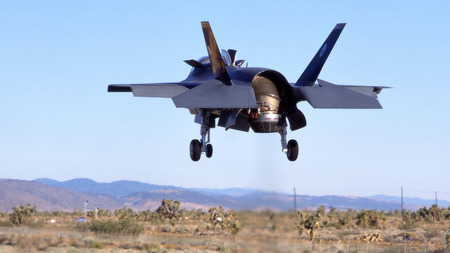
\includegraphics[width=0.45\textwidth]{figures/f35.jpg}
        \caption{F-35 Lighting II combat aircraft during take off}\label{f35}
      \end{figure}

\end{itemize}

The present work is centered on the analysis and study of multirotors, particularly on the modelling and control of a quadcopter carrying a manipulator arm. However, during the development of the project, the hexacopter configuration was also used. It allowed the obtention of some interesting results.

\section{Multi-rotors: state of the art}

The most common vehicle with the capacity of take off and landing in vertical way is the standard helicopter, which is composed of a principal rotor and a rear rotor. However, the multirotors, where we can find the four rotor helicopter, quadrotor or quadcopter, the hexacopter or hexarotor and the octocopter or octorotor have been the center of interest for many works in the last years, see \cite{Guerrero:2011}, \cite{Alaimo:2013} and \cite{Fogelberg:2008}. Some of the advantages offered by these vehicles are its symmetry, which makes it easy to design and build. The usage of four, six or eight rotors provides improved stability on hover, because the distributed pushing forces are acting at the same distance from the center of mass instead of just one pushing force acting on the whole center of mass. Also, the propellers can be protected by the frame of the prototype, which makes its usage indoor safer, face to the non-protected propellers of the standard helicopter.

The modeling of this kind of vehicles has done possible the design of many control laws which allow the attitude and position stabilization with good results. Some of the most used control laws have been: backstepping, found on \cite{Bouabdallah:2005}, \cite{Abdelaziz:2006} and \cite{Wu:2010}; sliding mode control has also been applied to these vehicles, and it can be found on \cite{Bouabdallah:2005}, \cite{Zheng:2014} and \cite{Arellano:2013}; linear control laws (PD and PID), they can be seen at \cite{erginer:2007}, \cite{li:2011} and \cite{hoffmann:2007}.

Other interesting projects developed with multi-rotors can be found on the domains of: navigation, where embedded cameras and/or different sensors are used to know the relative position of the aerial system, see \cite{courbon:2009} and \cite{sebesta:2012}; fault-tolerant control, where fault detection on the actuators is implemented and a control law is proposed for the aerial vehicle, see \cite{sharifi:2010} and \cite{li:2013}.




 \subsection{Characteristics and operation of the mini-UAV}

 \label{subsubsection:quadri}

 This part of the chapter is devoted to the mathematical modeling of the quadrotor. First, a general description of the function of the system is presented. After that, the mathematical modeling is treated, and equally the relation between motors, propellers and the dynamics of the system.

 The quadrotor or four rotor helicopter is a mechatronic system composed of a cross structure. At each end of the cross we find a propeller coupled to a motor, and at the center of the configuration all the electronic elements are found (power source, computer, etc). Compared to the classical helicopter, this system does not have main rotor and the control is performed by the angular velocity change on each rotor, \cite{Nelson:1998}.

 The four rotors are composed of the propellers coupled to DC motors or DC Brushless motors (BLDC). Such a platform is represented in \fig{fig:fourrotor}, where the front and rear motors (1 and 2) rotate clockwise, while the other two (3 and 4) rotate counterclockwise. In this way, gyroscopic effects and aerodynamic torques tend to cancel each other out in trimmed flight.
 \begin{figure}[h!]
     \centering
     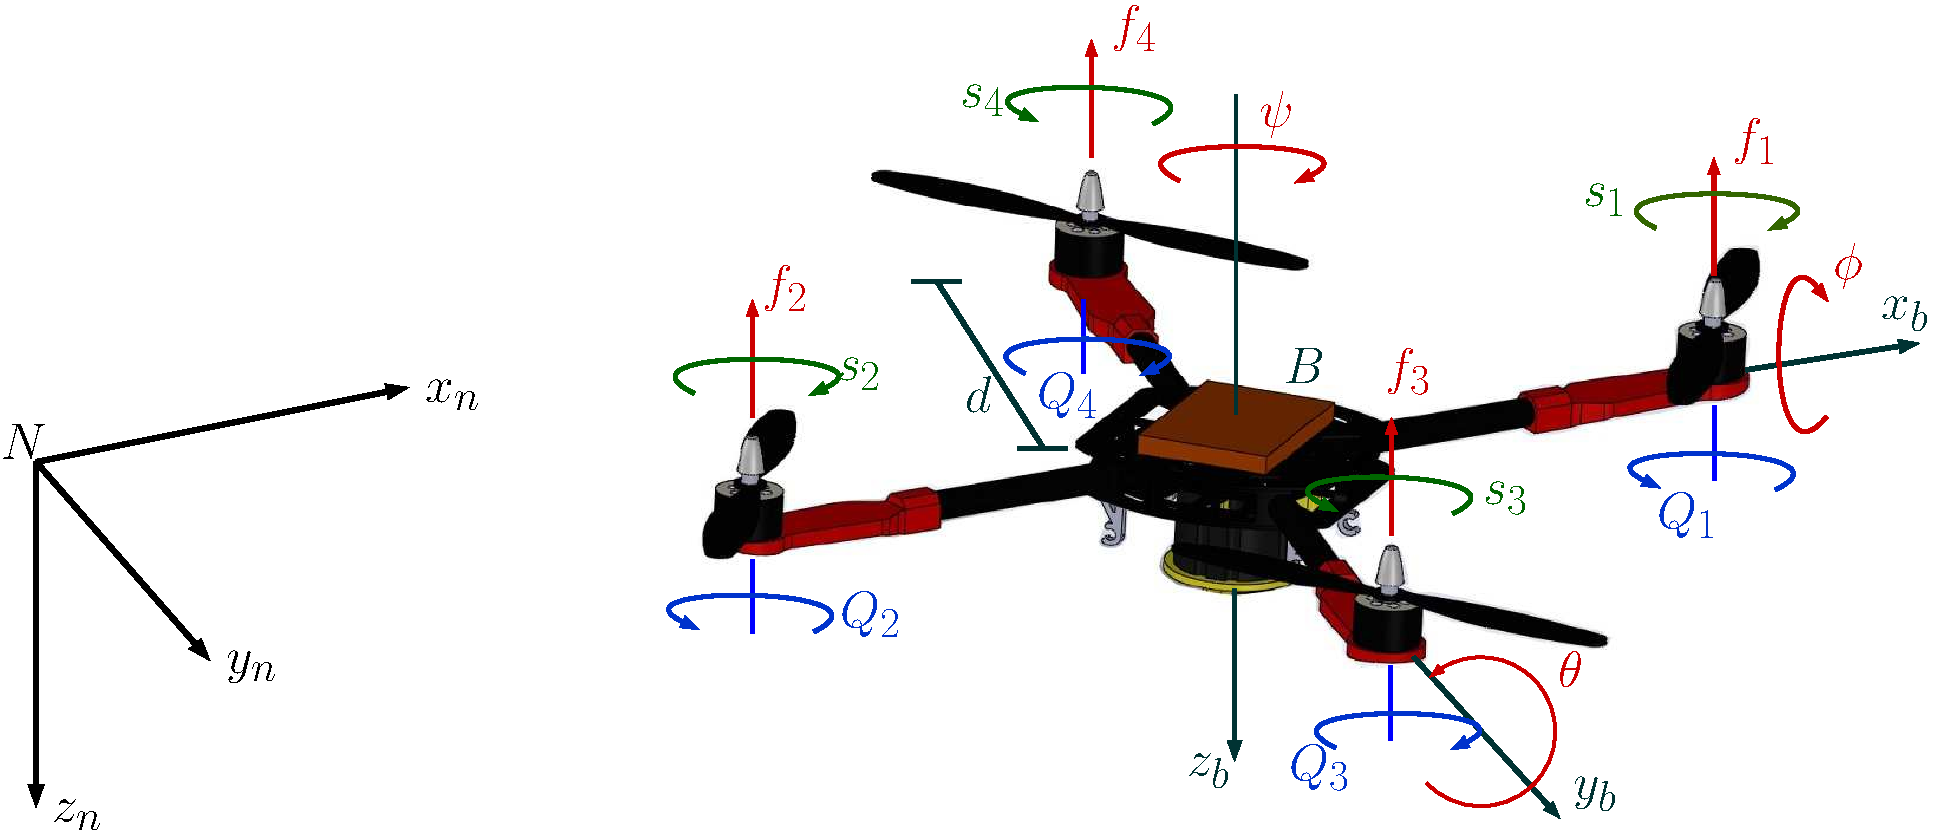
\includegraphics[width =0.9\textwidth]{figures/quadoperation.pdf}
     \caption{Scheme of the quadrotor configuration: inertial reference frame $N(x_n,y_n,z_n)$, the reference body fixed frame $B(x_b,y_b,z_b)$, the $f_i$ forces on each motor, angular velocity of the motors $s_{i}$ and the reaction torques $Q_i$.}
     \label{fig:fourrotor}
   \end{figure}

 Each rotor produces a force $f_i$ parallel to its rotation axe, as well as a drag torque $Q_i$, opposite to the direction of rotation. The total force or total thrust acting on the helicopter (parallel to the $z_b$ axis) is the addition of the four forces generated by each rotor $(F_T=f_1+f_2+f_3+f_4)$. The combination of these forces and the drag torques allow the angular motions over the main axes of the helicopter. Consequently, three movements for the position are produced, see \fig{fig:angmotion}.
 \begin{itemize}
   \item \textbf{Roll} ($\phi$): It is produced by the difference $f_3-f_4$. To obtain this, the velocity of the right motor $m_3$ is increased/reduced, while the velocity of the motor $m_4$ is equally decreased/increased. This difference of forces produces a torque $\Gamma_\phi$ around the axis $x_b$.
   \item \textbf{Pitch} ($\theta$): It is produced by the difference $f_1-f_2$. It is obtained similarly using the front and rear motors $m_1$ and $m_3$. This difference of forces produces a torque $\Gamma_\theta$ around the axis $y_b$.
   \item \textbf{Yaw} ($\psi$): It is the combination of all the reactive torques, $Q_1+Q_2-Q_3-Q_4$. It is obtained by decreasing/increasing the speed of the front and rear motors while decreasing/increasing the speed of the lateral motors. In other words, if a difference of speed between the motors turning in the opposite direction is produced, the reactive torques produce a torque $\Gamma_\psi$ around the axis $z_n$.
   \item \textbf{Vertical displacement on the $x_n$ axis}: To go forward or back, the rotational speed of motor $m_2$ must be decreased/increased, while decreasing/increasing the rotational speed of the motor $m_1$.
   \item \textbf{Lateral displacement on the $y_n$ axis}: To go to the right or left, the rotational speed of the lateral motors $m_4$ and $m_3$ must be decreased/increased.
   \item \textbf{Displacement on the $z_n$ axis}: To go up or down, the torque of all the rotors $m_i$ must be decreased/increased. In the absence of disturbances, the aerial system can perform a hover at a certain height by having a zero translation speed. Then, the total thrust $F_T$ must balance the weight $mg$ of the aerial system by pointing its direction in the axe $z_b$.
 \end{itemize}

 The first three movements are considered for the body fixed frame, and the last three for the inertial reference frame.
 \begin{figure}[h!]
     \centering
     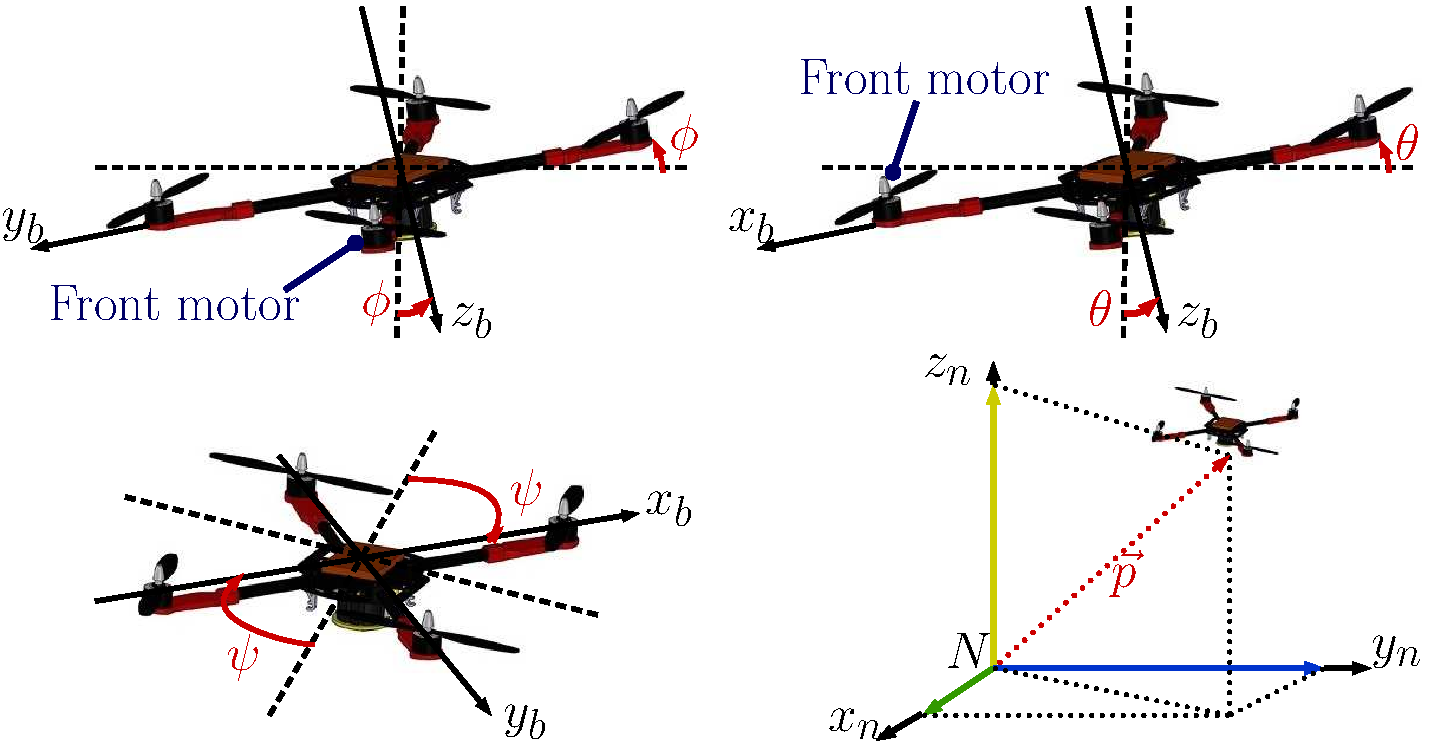
\includegraphics[width =0.8\textwidth]{figures/rollpitchyaw2.pdf}
     \caption{Roll ($\phi$), pitch ($\theta$), yaw ($\psi$) and space displacement}
     \label{fig:angmotion}
   \end{figure}

 From the description of the different angular movements and the vertical and horizontal displacements, it is visible that the position of the system depends on its attitude. In this way, the displacement of the quadcopter can be controlled from the attitude control.


 \section{Position representation}

 Robot tasks are often defined by the use of Cartesian coordinates. Let consider the scheme in \fig{fig:frame_pos}. It is possible to specify the coordinates of the point $p$ with respect to either frame $o_0x_0y_0$ or frame $o_1x_1y_1$.

 Geometrically, a point corresponds to a specific location in space, and a vector specifies a direction and a magnitude. Vectors can be used, for example, to represent displacements or forces. Therefore, while the point $p$ is not equivalent to the vector $\upsilon_1$, the displacement from the origin $o_0$ to the point $p$ is given by the vector $\upsilon_1$. Under this convention, it is clear that points and vectors are not equivalent, since points refer to specific locations in space, but a vector can be moved to any location in space. Then, two vectors are said to be equal if they have the same direction and the same magnitude.

 When assigning coordinates to vectors, the same notational convention is used as when assigning coordinates to points. Thus, $\upsilon_1$ and $\upsilon_2$ are geometric entities that are invariant with respect to the choice of coordinate systems, but the representation by coordinates of these vectors depend directly on the choice of reference coordinate frame.\\
 Using this convention, an expression of the form $\upsilon_1^1+\upsilon_2^2$ where $\upsilon_1^1$ and $\upsilon_2^2$ are as in \fig{fig:frame_pos}, is not defined since the frames $o_0x_0y_0$ and $o_1x_1y_1$ are not parallel. Thus, a clear need appears, not only for a representation system that allows points to be expressed with respect to various coordinate systems, but also for a mechanism that allows to transform the coordinates of points that are expressed in one coordinate system into the appropriate coordinates with respect to some other coordinate frame.
 \begin{figure}[h]
     \centering
     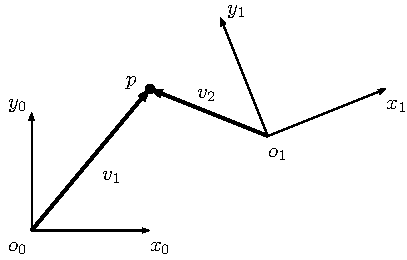
\includegraphics[width =0.5\textwidth]{figures/frame_pos.pdf}
     \caption{Two coordinate frames, a point $p$, and two vectors $\upsilon_1$ and $\upsilon_2$, (\cite{Spong:2004}).}
     \label{fig:frame_pos}
   \end{figure}

 \section{Rigid body attitude representation}

 Consider two orthogonal right-handed coordinate frames: the body coordinate frame, $B(x_b,y_b,z_b)$ located at the center of mass of the rigid body and the inertial coordinate frame, $N(x_n,y_n,z_n)$, located at some point in the space (for instance, the earth NED frame). This coordinate system is showed in \fig{fig:inertial_fixed}. In general, the origin of $B$ is chosen to coincide with the gravity center (CG) of the body.

 The body attitude in the space can be represented in many ways, each one with their advantages and disadvantages, depending mainly on the application.
 \begin{figure}[H]
     \centering
     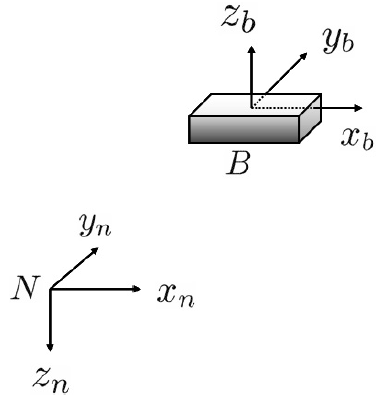
\includegraphics[width =0.28\textwidth]{figures/inertial_fixed.png}
     \caption{Inertial and mobile frame of a rigid body.}
     \label{fig:inertial_fixed}
   \end{figure}

 \begin{definition}
 The movement of a rigid body with reference frame B relative to a rigid body or reference frame N is called a simple rotation of B in N, if there is a line L, called rotation axis, where the orientation relative to B and N keeps the same between the start and the end of the movement.
 \end{definition}
 \begin{theorem}
    (Rotation Euler Theorem). Every relative change in orientation between two rigid bodies with the two coordinate systems B and N can be produced by one simple rotation of B over N.
 \end{theorem}
 Let $\vec{b}$ and $\vec{r}$ be the coordinates of a vector $\vec{X}$ in $B$ and $N$ respectively. Vector $\vec{b}$ can be written in terms of vector $\vec{r}$.

 Let $\vec{e} = [e_1\,\, e_2\,\, e_3]$ be a unit vector collinear to the rotation axis $L$ around which $B$ is rotated by an angle $\beta$. Consequently, $\vec{b}$ is obtained by
 \begin{equation}\label{eq:b}
 \vec{b} = \cos \beta \vec{r} + (1 - \cos \beta)\vec{e}\ \vec{e}\ ^T\vec{r} - \sin\beta\vec{e} \times \vec{r}
 \end{equation}
 In fact, the coordinates $\vec{b}$ and $\vec{r}$ are linked by means of the following linear transformation:
 \begin{equation}
 \vec{b} = C\vec{r}
 \end{equation}
 Matrix $C$ can be token as an operator which takes a fixed vector $\vec{r}$ expressed in $N$ and is expressed in $B$. From (\ref{eq:b})
 \begin{equation}
 C = \cos\beta I_3 + (1 - \cos\beta)\vec{e}\ \vec{e}\ ^T - \sin\beta[\vec{e}\ ^\times]
 \end{equation} where $I_3$ represents the identity matrix of dimension three and $[\xi^\times]$ represents the skew-symmetric matrix, given by:
 \begin{equation}\label{skew}
   [\xi^\times]=\left(\begin{array}{c}
                  \xi_1 \\
                  \xi_2 \\
                  \xi_3
                \end{array}\right)^\times=\left(
                                                  \begin{array}{ccc}
                                                    0 & \xi_3 & \-\xi_2 \\
                                                    -\xi_3 & 0 & \xi_1 \\
                                                    \xi_2 & -\xi_1 & 0 \\
                                                  \end{array}\right)
 \end{equation}
 Matrix $C \in \mathbb{R}^{3\times3}$ identifies the orientation of the moving frame $B$ with respect to the inertial frame $N$ and it allows the coordinate transformation of a vector system into another one. This matrix is known as the direction cosine matrix (DCM), rotation matrix or attitude matrix.

 \subsubsection{Rotation matrix}

 Rotation matrix $C$ belongs to the subspace of orthogonal matrices of dimension three, called special orthogonal group, denoted by $S0(3)$, and defined by
 \begin{equation}\label{so3}
   S0(3)={C|C\in \mathbb{R}^{3\times3},C^TC=I_3,\det(C)=1}
 \end{equation}
 In a rotation matrix $C$, each element $c_{ij}$ is a direct cosine, given by:
 \begin{equation}\label{C}
   C=\left(
       \begin{array}{ccc}
         c_{11} & c_{12} & c_{13} \\
         c_{21} & c_{22} & c_{23} \\
         c_{31} & c_{32} & c_{33} \\
       \end{array}\right)
 \end{equation} where
 \begin{equation}\label{cij}
   c_1=\left(
         \begin{array}{c}
           c_{11} \\
           c_{21} \\
           c_{31} \\
         \end{array}\right)\ \ c_1=\left(
         \begin{array}{c}
           c_{12} \\
           c_{22} \\
           c_{32} \\
         \end{array}\right)\ \ c_1=\left(
         \begin{array}{c}
           c_{13} \\
           c_{23} \\
           c_{33} \\
         \end{array}\right)
 \end{equation}
 Consequently,
 \begin{equation}\label{C2}
   C=\left(
       \begin{array}{ccc}
         c_1 & c_2 & c_3 \\ \end{array}\right)
 \end{equation} where
 \begin{equation}
   c_i^Tc_i=1\ \ \textrm{and}\ \ c_i^Tc_j=0\ \ \forall i\neq j
 \end{equation}

 \subsubsection{Rotational velocity}

 Suppose that a rotation matrix $C$ is time varying, so that $C=C(t)\ \in\ S0(3)$ for every $t\ \in\ \mathbb{R}$. Assuming that $C(t)$ is continuously differentiable as a function of $t$. An argument identical to the one in the previous section shows that the time derivative $\dot{C}(t)$ of $C(t)$ is given by
 \begin{equation}
   \dot{C}(t)=[\vec{\omega}\ ^\times]C(t)
 \end{equation} where $\vec{\omega}$ is the angular velocity of the rotating frame with respect to the fixed frame at time $t$.

 \subsubsection{Euler angles and Roll, Pitch and Yaw angles}
 \begin{figure}[H]
     \centering
     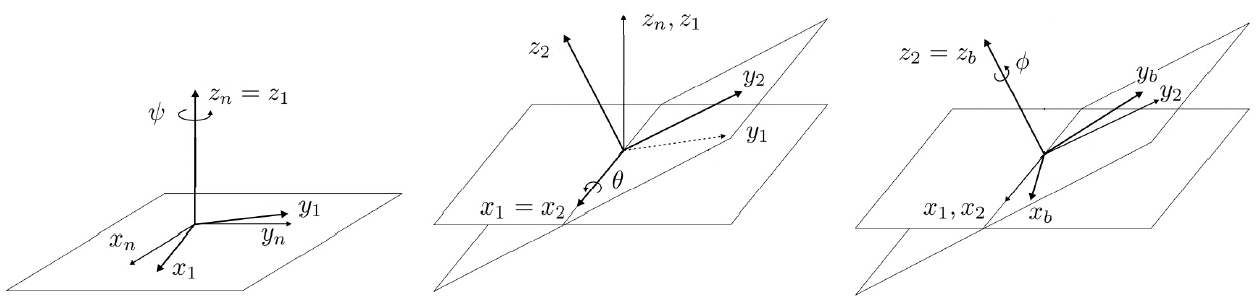
\includegraphics[width =\textwidth]{figures/euler.png}
     \caption{Euler angles.}
     \label{fig:euler_an}
   \end{figure}

 A common method of specifying a rotation matrix in terms of three independent quantities is to use the so-called Euler Angles $(\psi,\theta,\varphi)$. Consider again the fixed coordinate frame $N(x_n,y_n,z_n)$ and the rotated frame $(x_b,y_b,z_b)$, shown in \fig{fig:euler_an}.

 It is possible to specify the orientation of the frame $(x_1,y_1,z_1)$ relative to the frame $N(x_n,y_n,z_n)$ by the three angles, and it can be obtained by three successive rotations as follows: first rotate about z-axis by the angle $\phi$, next, rotate about the current y-axis by the angle $\theta$. Finally, rotate about the current z-axis by the angle $\psi$.
 In terms of the basic rotation matrices the resulting rotational transformation $C_1^0$ can be generated as the product
 \begin{equation}\label{euler}
 \begin{split}
 C_1^0=C_{z,\phi},C_{y,\theta},C_{z,\psi} &= \left[\begin{array}{ccc}
                                                      c_\phi & -s_\phi & 0 \\
                                                      s_\phi & c_\psi & 0 \\
                                                      0 & 0 & 1 \end{array}\right]\left[\begin{array}{ccc}
                                                                                          c_\theta & 0 & s_\theta \\
                                                                                          0 & 1 & 0 \\
                                                                                          -s_\theta & 0 & c_\theta \end{array}\right]\left[\begin{array}{ccc}
                                                                                                                    c_\psi & -s_\psi & 0 \\
                                                                                                                    s_\psi & c_\psi & 0 \\
                                                                                                                     0& 0 & 1
                                                                                                                  \end{array}
                                                                                          \right]\\
                                                      &=\left[\begin{array}{ccc}
                                                        c_\phi c_\theta c_\psi-s_\phi s_\psi & -c_\phi c_\theta s_\psi-s_\phi c_\psi & c_\phi s_\theta \\
                                                        s_\phi c_\theta c_\psi+c_\phi s_\psi & -s_\phi c_\theta s_\psi+c_\phi c_\psi & s_\phi s_\theta \\
                                                        -s_\theta c_\psi & s_\theta s_\psi & c_\theta                     \end{array}\right]
 \end{split}
 \end{equation}

 A rotation matrix $C$ can also be described as a product of successive rotations about the principal coordinate axes $x_n$, $y_n$ and $z_n$ taken in a specific order. These rotations define the roll, pitch and yaw angles. The order of rotations is specified as $z-y-x$, in other words, first a yaw about $z_n$ by an angle $\phi$, then pitch about the $y_n$ by an angle $\theta$, and finally roll about the $x_n$ by an angle $\psi$. Since the successive rotations are relative to the fixed frame, the resulting transformation matrix is given by
 \begin{equation}\label{euler}
 \begin{split}
   C_1^0=C_{z,\phi}C_{y,\theta}C_{x,\psi}&=\left[\begin{array}{ccc}
                                                   c_\phi & -s_\phi & 0 \\
                                                   s_\phi & c_\phi & 0 \\
                                                   0 & 0 & 1
                                                 \end{array}
   \right]\left[\begin{array}{ccc}
                  c_\theta & 0 & s_\theta \\
                  0 & 1 & 0 \\
                  -s_\theta & 0 & c_\theta
                \end{array}\right]\left[\begin{array}{ccc}
                                          1 & 0 & 0 \\
                                          0 & c_\psi & -s_\psi \\
                                          0 & s_\psi & c_\psi
                                        \end{array}\right] \\
                                        &=\left[\begin{array}{ccc}
                                                c_\phi c_\theta & -s_\phi c_\psi+c_\phi s_\theta s_\psi & s_\phi s_\psi+c_\phi s_\theta c_\psi \\
                                                s_\phi c_\theta & c_\phi c_\psi+s_\phi s_\theta s_\psi & -c_\phi s_\psi+s_\phi s_\theta c_\psi \\
                                                -s_\theta & c_\theta s_\psi & c_\theta c_\psi
                                              \end{array}\right]
 \end{split}
 \end{equation}

 Now, let $\vec{\omega}=[\begin{array}{ccc}\omega_x & \omega_y & \omega_z\end{array}]$ be the angular velocity of the body in the reference frame $B$ with respect to the reference frame $N$. Then, the kinematic equation is given by \cite{Fossen:1994}:
 \begin{equation}\label{vitesse}
   \left(\begin{array}{c}
           \dot{\phi} \\
           \dot{\theta} \\
           \dot{\psi}\end{array}\right)=\left(\begin{array}{ccc}
                                                1 & \tan\theta\sin\phi & \tan\theta\sin\phi \\
                                                0 & \cos\phi & -\sin\phi \\
                                                0 & \frac{\sin\phi}{\cos\theta} & \frac{\cos\phi}{\cos\theta}
                                              \end{array}\right)\left(\begin{array}{c}
                                                                        \omega_x \\
                                                                        \omega_y \\
                                                                        \omega_z
                                                                      \end{array}
                                              \right)
 \end{equation}

 \subsubsection{Quaternions}

 The drawbacks of the angle/axis representation can be overcome by a different four-parameter representation; namely, the unit \emph{quaternion} or Euler parameters, defined by:
 \begin{equation}\label{defquaternion}
         q:=\left(%
 \begin{array}{c}
   \cos \frac{\beta}{2} \\
   \vec{e} \sin \frac{\beta}{2}  \\
 \end{array}%
 \right)=\left(\begin{array}{c}
   q_0 \\
   q_v  \\
 \end{array}\right)   \in \mathbb H
 \end{equation} where
 \begin{equation}\label{H}
   \mathbb H={q|q_0^2+\vec{q}\ ^T\vec{q}=1, \ q=\left(\begin{array}{c}
   q_0 \\
   \vec{q}  \\
 \end{array}\right), \ q_0\in\mathbb{R}, \ \vec{q}\in\mathbb{R}^3}
 \end{equation} where $\vec{q}=(q_1\ \ q_2 \ \ q_3)^T \in \mathbb R^3 $ and $q_0 \in \mathbb R$ are known as the vector and scalar parts of the quaternion respectively. The identity quaternion and the conjugated quaternion are given by:
 \begin{equation}\label{qid}
   q_{id}=[1 \ \ 0^T]\ ^T \ \ \bar{q}=[q_0 \ \ -\vec{q}\ ^T]\ ^T
 \end{equation}
 Since the quaternion is unitary, $q^{-1}=\bar{q}$.
 The product of two quaternions $q_1=[q_{1_{0}} \ \ \vec{q_1}^T]^T$ and $q_2=[q_{2_{0}} \ \ \vec{q_2}^T]^T$ is defined by:
 \begin{equation}\label{multiq}
   q_1\otimes q_2=\left(\begin{array}{cc}
                          q_{1_{0}} & -\vec{q}_1\ ^T \\
                          \vec{q}_1 & I_3q_{1_{0}}+[\vec{q}\ ^\times]
                        \end{array}\right)\left(\begin{array}{c}
                                                  q_{2_{0}} \\
                                                  \vec{q}_2 \end{array}\right)
 \end{equation}

 Now, let $b_q$ and $r_q$ be the quaternions associated to vectors $\vec{b}$ and $\vec{r}$, defined by:
 \begin{equation}
   b_q=[0 \ \ \vec{b}\ ^T]\ ^T \ \ r_q=[0 \ \ \vec{r}\ ^T]\ ^T
 \end{equation}
 These two quaternions are linked by the next relation:
 \begin{equation}
   b_q=q\otimes r_q \otimes q^{-1}=q \otimes r_q \otimes \bar{q}
 \end{equation}

 Rotation matrix $C$ can be expressed in terms of quaternions by:
 \begin{equation}\label{rotq}
   C=C(q)=(q_0^2-\vec{q}\ ^T\vec{q})I_3+2(\vec{q}\ \vec{q}\ ^T-q_0[\vec{q}\ ^\times])
 \end{equation} from where
 \begin{equation}\label{Cq}
   C(q)=\left(\begin{array}{ccc}
                2(q_0^2+q_1^2)-1 & 2(q_1q_2+q_0q_3) & 2(q_1q_3-q_0q_2) \\
                2(q_1q_2-q_0q_3) & 2(q_0^2+q_2^2)-1 & 2(q_0q_1+q_2q_3) \\
                2(q_0q_2+q_1q_3) & 2(q_2q_3-q_0q_1) & 2(q_0^2+q_3^2)-1 \end{array}\right)
 \end{equation}

 The relation between the vectors $\vec{b}$ and $\vec{r}$ is:
 \begin{equation}
   \vec{b}=C(q)\vec{r}
 \end{equation}
 Denoting by $w=(\omega_1\ \ \omega_2\ \ \omega_3)^T$ the angular velocity vector of the body coordinate frame, $B$ relative to the inertial  coordinate frame $N$ expressed in $B$, the kinematics equation is given by
 \begin{equation}\label{eqkinematic}
 \left(%
 \begin{array}{c}
   \dot{q}_0 \\
   \dot{\vec{q}} \\
 \end{array}%
 \right) =  \frac{1}{2}\left(%
 \begin{array}{c}
   -\dot{q}^T \\
   I_3q_0 + [\vec{q}^\times] \\
 \end{array}%
 \right) w=\frac{1}{2}\Xi(q)w
 \end{equation}

 \subsubsection{Rigid motions}

 \begin{definition}
   A rigid motion is an ordered pair (d,C) where $d\ \in\ \mathbb{R}^3$ and $C\ \in\ SO(3)$. The group of all rigid motions is known as the \textbf{Special Euclidean Group} and is denoted by $SO(3)$. It is denoted that $SO(3)=\mathbb{R}^3\times SO(3)$.
 \end{definition}

 A rigid motion is a pure translation together with a pure rotation.

 \subsubsection{Homogeneous transformations}

 The combination of position and orientation representations allows the formulation of homogeneous transformations, used in the modeling of arm manipulators. Then, the transformation matrices with the form:
 \begin{equation}\label{eq:homo}
   H=\left[\begin{array}{cc}
             C & d \\
             0 & 1 \end{array}\right]
 \end{equation} are called \textbf{homogeneous transformations}. Then, a homogeneous transformation is a representation of a rigid motion where the system $S0(3)$ is used interchangeably to represent the set of rigid motions and the set of all $4\times4$ matrices given in (\ref{eq:homo}).

 A set of basic homogeneous transformations generating $S0(3)$ is given by
 \begin{equation}\label{transx}
   Trans_{x,a}=\left[\begin{array}{cccc}
                       1 & 0 & 0 & a \\
                       0 & 1 & 0 & 0 \\
                       0 & 0 & 1 & 0 \\
                       0 & 0 & 0 & 1 \end{array}\right];\ \ Rot_{x,a}\left[\begin{array}{cccc}
                                                                            1 & 0 & 0 & 0 \\
                                                                            0 & c_a & -s_a & 0 \\
                                                                            0 & s_a & c_a & 0 \\
                                                                            0 & 0 & 0 & 1 \end{array}\right]
 \end{equation}
 \begin{equation}\label{transx}
   Trans_{y,b}=\left[\begin{array}{cccc}
                       1 & 0 & 0 & 0 \\
                       0 & 1 & 0 & b \\
                       0 & 0 & 1 & 0 \\
                       0 & 0 & 0 & 1 \end{array}\right];\ \ Rot_{y,b}\left[\begin{array}{cccc}
                                                                            c_\beta & 0 & s_\beta & 0 \\
                                                                            0 & 1 & 0 & 0 \\
                                                                            -s_\beta & 0 & c_\beta & 0 \\
                                                                            0 & 0 & 0 & 1 \end{array}\right]
 \end{equation}
 \begin{equation}\label{transx}
   Trans_{z,c}=\left[\begin{array}{cccc}
                       1 & 0 & 0 & 0 \\
                       0 & 1 & 0 & 0 \\
                       0 & 0 & 1 & c \\
                       0 & 0 & 0 & 1 \end{array}\right];\ \ Rot_{x,a}\left[\begin{array}{cccc}
                                                                            c_\gamma & -s_\gamma & 0 & 0 \\
                                                                            s_\gamma & c_\gamma & 0 & 0 \\
                                                                            0 & 0 & 1 & 0 \\
                                                                            0 & 0 & 0 & 1 \end{array}\right]
 \end{equation} for translation and rotation about the $x,y,z$ axis respectively.\\
 The most general homogeneous transformation that is considered is given by
 \begin{equation}\label{homogen}
   H_1^0=\left[\begin{array}{cccc}
                 n_x & s_x & a_x & d_x \\
                 n_y & s_y & a_y & d_y \\
                 n_z & s_z & a_z & d_z \\
                 0 & 0 & 0 & 1 \end{array}\right]=\left[\begin{array}{cccc}
                                                          n & s & a & d \\
                                                          0 & 0 & 0 & 1 \end{array}\right]
 \end{equation}
 In the above equation $n=(n_x,n_y,n_z)^T$ is a vector representing the direction of $X_1$ in the $o_0x_0y_0$ system, $s=(s_x,s_y,s_z)^T$ represents the direction of $y_1$, and $a=(a_x,a_y,a_z)$ represents the direction of $z_1$. $d=(d_x,d_y,d_z)^T$ represents the vector from the origin $o_0$ to the origin $o_1$ expressed in the frame $o_0x_0y_0z_0$.

 \subsubsection{Attitude error}

 Two orientations of a rigid body are considered, described by rotation matrices $C_1$ and $C_2$ respectively. Then, the relative attitude between these two orientations is computed by:
 \begin{equation}\label{Cr}
   C_r=C_1^{-1}C_2
 \end{equation}
 In fact, $C_r$ represents an operator of orientation which rotates $C_2$ about $C_1$. From here, the relative orientation is used in the estimation and in the orientation control as \emph{attitude error}. With this, $C_d=C_1$ is the desired attitude of a rigid body and $C=C_2$ is the real attitude of the body.
 Consequently, the attitude error is computed by:
 \begin{equation}\label{Ce}
   C_e=C_d^{-1}C
 \end{equation}
 If the attitude error is zero, then, $C_e=I_3$.
 When the unitary quaternion is used to represent the attitude of the body, the relative orientation between $q_1$ and $q_2$ is expressed by:
 \begin{equation}\label{qr}
   q_r=q_1^{-1}\otimes q_2=\left(\begin{array}{cc}
                                  q_{1_{0}} & \vec{q}_1\ ^T \\
                                  -\vec{q}_1 & I_3q_{1_{0}}-[\vec{q}\ ^\times]\end{array}
   \right)\left(\begin{array}{c}
                  q_{2_0} \\
                  \vec{q}_2 \end{array}\right)=\bar{q}_1\otimes q_2
 \end{equation}
 The geodesic metric is given by the next expression:
 \begin{equation}\label{betar}
   \beta_r=2|\arccos(q_{r_{0}})|
 \end{equation}
 This metric represents the smallest angle of rotation between attitude $q_1$ and the attitude $q_2$. The Euclidean distance between the two unitary quaternions gives an approximation of the geodesic metric:
 \begin{equation}\label{geodesic}
   \frac{2}{\pi}\beta_r\leq2\parallel q_1-q_2\parallel_2\leq\beta_r
 \end{equation}
 Also, when $\beta_r$ is enough small, it is possible to do the next approximation:
 \begin{equation}\label{approx}
   \beta_r\approx2\parallel q_1-q_2\parallel_2
 \end{equation}

 For the case of the attitude control law, if $q_d=q_1$ is the desired attitude of the body and $q=q_2$ is the real attitude of the body, the attitude error is given by:
 \begin{equation}\label{qerr}
   q_e=q_d^{-1}\otimes q=\bar{q}_d\otimes q
 \end{equation}
 When the attitude error is zero, the error quaternion has two possible values:
 \begin{equation}\label{qe1}
   q_e=[\pm1 \ \ 0]^T
 \end{equation}
 This is due to the non bijection quaternion with the group $SO(3)$.

% \subsection{Notation and axis system}
% \subsection{Dinamic model of a mini-UAV}

 \section{Conclusions}
